% --------------------------------------------------------------
% This is all preamble stuff that you don't have to worry about.
% Head down to where it says "Start here"
% --------------------------------------------------------------
 
\documentclass[12pt]{article}
 
\usepackage[margin=1in]{geometry} 
\usepackage{amsmath,amsthm,amssymb,listings,xcolor,graphicx,framed,subfig}
\usepackage{booktabs}
 
\newcommand{\N}{\mathbb{N}}
\newcommand{\Z}{\mathbb{Z}}
 
\newenvironment{theorem}[2][Theorem]{\begin{trivlist}
\item[\hskip \labelsep {\bfseries #1}\hskip \labelsep {\bfseries #2.}]}{\end{trivlist}}
\newenvironment{lemma}[2][Lemma]{\begin{trivlist}
\item[\hskip \labelsep {\bfseries #1}\hskip \labelsep {\bfseries #2.}]}{\end{trivlist}}
\newenvironment{exercise}[2][Exercise]{\begin{trivlist}
\item[\hskip \labelsep {\bfseries #1}\hskip \labelsep {\bfseries #2.}]}{\end{trivlist}}
\newenvironment{problem}[2][Problem]{\begin{trivlist}
\item[\hskip \labelsep {\bfseries #1}\hskip \labelsep {\bfseries #2.}]}{\end{trivlist}}
\newenvironment{question}[2][Question]{\begin{trivlist}
\item[\hskip \labelsep {\bfseries #1}\hskip \labelsep {\bfseries #2.}]}{\end{trivlist}}
\newenvironment{corollary}[2][Corollary]{\begin{trivlist}
\item[\hskip \labelsep {\bfseries #1}\hskip \labelsep {\bfseries #2.}]}{\end{trivlist}}

\newenvironment{solution}{\begin{proof}[Solution]}{\end{proof}}

\definecolor{codegreen}{rgb}{0,0.6,0}
\definecolor{codegray}{rgb}{0.5,0.5,0.5}
\definecolor{codepurple}{rgb}{0.58,0,0.82}
\definecolor{backcolour}{rgb}{0.97,0.97,0.97}
\lstdefinestyle{pystyle}{
    backgroundcolor=\color{backcolour},   
    commentstyle=\color{codegreen},
    keywordstyle=\color{magenta},
    numberstyle=\tiny\color{codegray},
    stringstyle=\color{codepurple},
    basicstyle=\ttfamily\tiny\tiny,
    breakatwhitespace=false,         
    breaklines=true,                 
    captionpos=b,                    
    keepspaces=true,                 
    numbers=left,                    
    numbersep=5pt,                  
    showspaces=false,                
    showstringspaces=false,
    showtabs=false,                  
    tabsize=2
}
\lstset{style=pystyle}

\graphicspath{{./figures}}
 
\begin{document}
 
\title{Problem Design: mmWave Arrays + Space Hardening}
\author{Matthew Luyten\\ %replace with your name
ECE8803}

\maketitle

\begin{enumerate} 
    \Large\item[I.] mmWave Arrays
    \normalsize
    
    \textbf{Title:} Designing mmWave Antenna Arrays on Silicon

    \textbf{Competency:} Understand some of the design constraints in designing mmWave antenna arrays on silicon.

    \textbf{Problem:}
    
    \begin{enumerate}
        \item[a.] On-chip integration of mmWave antennas has become increasingly common. List one benefit of integrating an antenna
        into an integrated circuit package besides miniaturization / reduction in footprint.

        \vspace{3cm}

        \item[b.] Below are three cross sections of mmWave dipole radiators as described by Fig. 1 on different substrates with varying relative permittivity ($\epsilon_r$). 
        Assume each the dipole is ideal with length $\frac{\lambda}{2}$. Sketch the radiation pattern for each radiator/substrate combination.

        \begin{figure}[!ht]
            \centering
            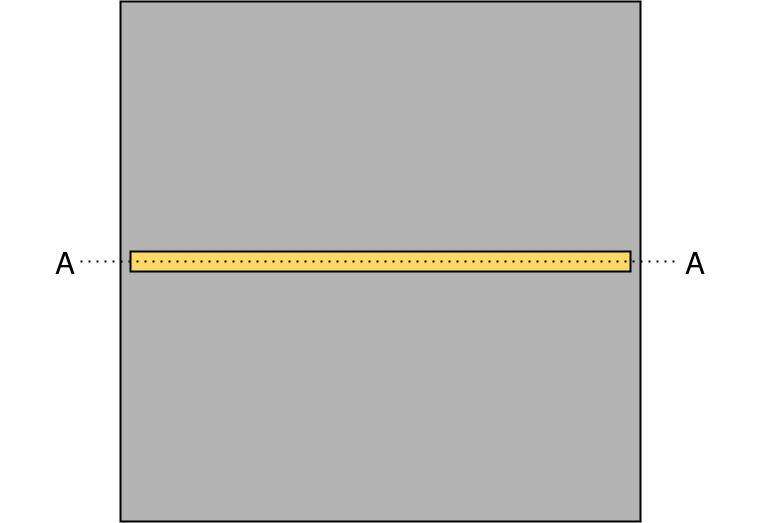
\includegraphics[width=2in]{crossection.png}
            \caption{Dipole Antenna with Cross Section}
        \end{figure}

        \clearpage

        \phantom{}

        \vspace{3.5cm}

        \begin{figure}[!ht]
            \centering
            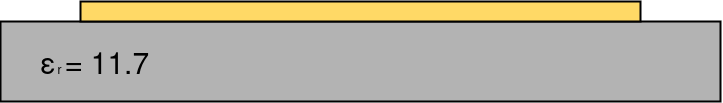
\includegraphics[width=3.5in]{ex1.png}
        \end{figure}

        \vspace{4cm}

        \begin{figure}[!ht]
            \centering
            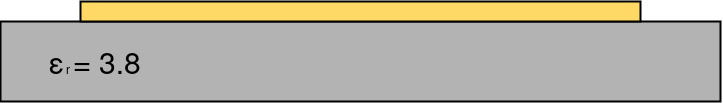
\includegraphics[width=3.5in]{ex2.png}
        \end{figure}

        \vspace{4cm}

        \begin{figure}[!ht]
            \centering
            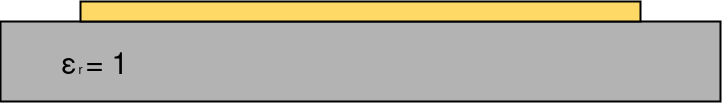
\includegraphics[width=3.5in]{ex3.png}
        \end{figure}

        \vspace{1cm}

        \clearpage

        \item[c.] You are tasked with designing an array of half-wave dipoles like those described in part b. This array must be designed on silicon as an on-chip antenna,
        and therefore, the substrate will be silicon ($\epsilon_r = 11.7$). Based on your answers from part b, what makes this a difficult design?
        How might you address the problem of using a substrate with such high permittivity?

        \vspace{3cm}

        \item[d.] You learn that your array must be a 3-element linear array, with a 45-degree phase shift between each element. Sketch a feed network
        for this array and label any important lengths in terms of $\lambda$. Explain your methodology and some design considerations.

        \begin{figure}[!ht]
            \centering
            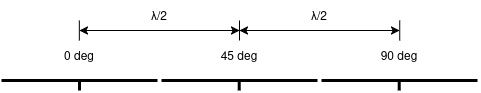
\includegraphics[width=5in]{feed.png}
        \end{figure}
    \end{enumerate}
    
    \newpage

    \textbf{Solution}

    \begin{enumerate}
        \item[a.] Correct answers incldude elimination of flip-chip interconnection loss, increased fabrication precision, decreased insertion loss, or 
        low power needs. 

        
        \item[b.] Perfect toroidal cross section not required. Correct answers should identify the relationship
        between directivity and the permittivity of the microstrip substrate. See example answer in Fig. 2.

        \begin{figure}[!ht]
            \centering
            \subfloat[]{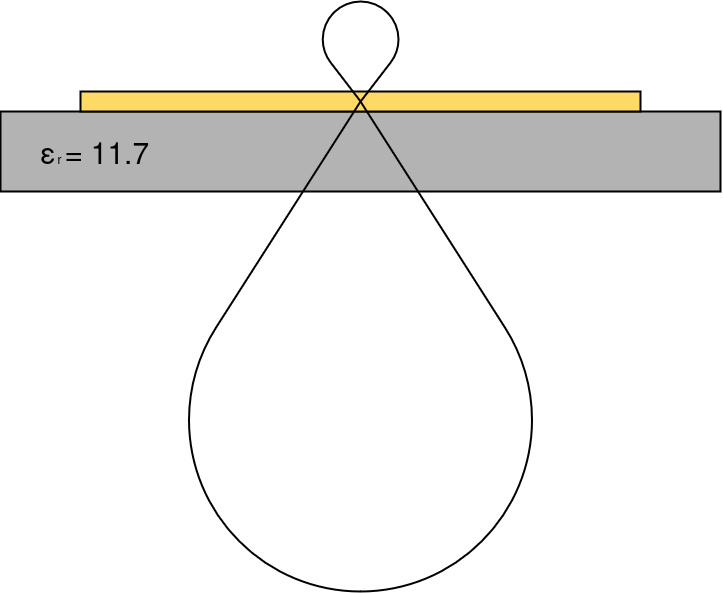
\includegraphics[width=2in]{ex1-sol.png}}
            \subfloat[]{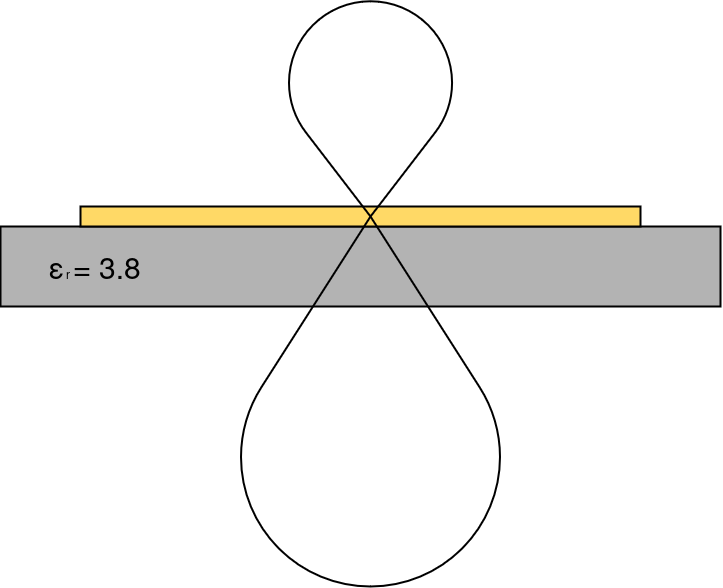
\includegraphics[width=2in]{ex2-soln.png}}
            \subfloat[]{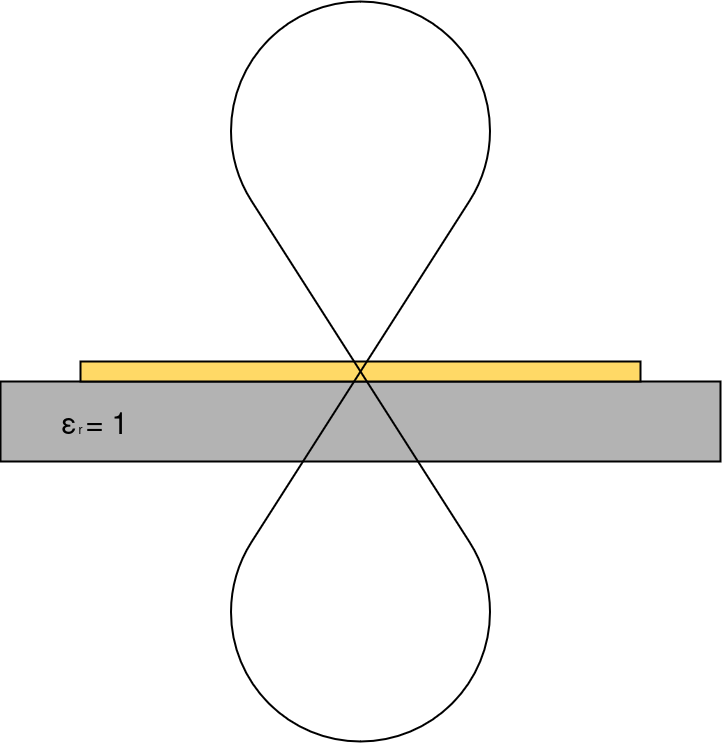
\includegraphics[width=2in]{ex3-soln.png}}
            \caption{Example Radiation Patterns for Part B}
        \end{figure}

        \item[c.] Correct answers identify that the directivity is increased in the direction of the dielectric. Solutions for this problem include:
        using a ground plane as a passive reflector, placing intermediate substrate with lower permittivity between the patch and the silicon, using a
        superstrate and posts to increase directivity away from the substrate, and fabricating a lense and using the substrate to focus the beam.

        \newpage
        
        \item[d.] Correct answers explain that phase shifters on mmWave silicon arrays may be too large or cost prohibitive. Design should use variable
        transmission line lengths to achieve desired phase shift. See example solution in Fig. 3. Bonus points if techniques to keep the wavefront 
        parallel to the transmission line, like air bridges, are mentioned. 
        
        \begin{figure}[!ht]
            \centering
            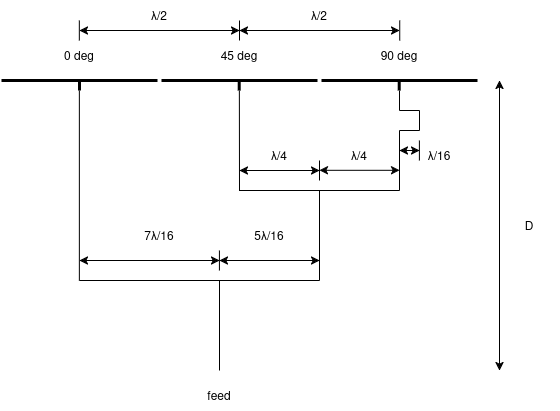
\includegraphics[width=5in]{feed-soln.png}
            \caption{Example Feed Network for Part D}
        \end{figure}

    \end{enumerate}

    \newpage

    \Large\item[II.] Space Hardening
    \normalsize
    
    \textbf{Title:} Space is RAD

    \textbf{Competency:} Understand the basics of the space radiation environment.

    \textbf{Problem:} 

    \begin{enumerate}
        \item[a.] What are the three main sources of radiation to be considered when designing a satellite?
        
        \vspace{3cm}

        \item[b.] Rank each locations from 1 - highest annual radiation dose to 7 - lowest annual radiation dose. Justify your ranking.
        \vspace{0.5cm}

        \_\_\_ High Inclination LEO Orbit

        \_\_\_ Low Inclination MEO Orbit

        \_\_\_ JPL Factory

        \_\_\_ Voyager Two's Current Location

        \_\_\_ Low Inclination LEO Orbit

        \_\_\_ Tundra Orbit

        \_\_\_ GSO Orbit

        \vspace{3cm}

        \item[c.] What are the two main ways that radiation damages semiconductors?
        
        \newpage

        \item[d.] You are designing the memory for a cubesat flying in LEO. Based on previous missions in the same orbit ,
        you know that high energy particles that cause bit upsets strike a $1 mm^2$ area according to a poisson 
        process with $\lambda = 0.0025/$ strikes per day. What is the probability that zero strikes occur during the first
        10 days? 
        
        \vspace{3cm}

        Based on your previous analysis, you determine that the memory must have some error correction. You design a scheme that
        can reverse any single bit flips. However, to identify flipped bits, you must read the data. If more than one bit flips occurs,
        the data is permanently corrupted. You decide that the processor must check for upsets every 8 hours to ensure the data is intact.
        What is the probability that the time between successive strikes is less than 8 hours? Based on your results, should you pursue other error
        correction schemes?

    \end{enumerate}

    \newpage

    \textbf{Solution}

    \begin{enumerate}
        \item[a.] The main sources of radiation that concern satellite operation are galactic cosmic rays, solar radiation/wind/flares/CME, 
        and high energy particles in the Van Allen belts.
        \vspace{0.5cm}

        \item[b.] Rank each locations from 1 - highest annual radiation dose to 7 - lowest annual radiation dose. Justify your ranking.
        \vspace{0.5cm}

        \_5\_ High Inclination LEO Orbit

        \_4\_ Low Inclination MEO Orbit

        \_7\_ JPL Factory

        \_1\_ Voyager Two's Current Location

        \_6\_ Low Inclination LEO Orbit

        \_2\_ Tundra Orbit

        \_3\_ GSO Orbit
        \vspace{0.5cm}

        We know the heliosphere protects the solar system from the majority of cosmic rays in deep space. However, it may be argued
        that the Tundra or GSO orbits receive more annual radiation from the sun or the Van Allen belts than the Voyager 2 does 
        outside of the heliosphere. It could also be argued that a low inclination MEO satellite may experience more radiation than
        a high-inclination LEO satellite if it was positioned directly in the inner Van Allen belt.
        \vspace{0.5cm}
        
        \item[c.] Semiconductors are damaged either by junction degradation from a total ionizing dose or upset/latch-up from a single
        event effect (i.e. a strike from a high-energy particle).

        \vspace{0.5cm}

        \item[d.] Given the RAM module has an area of $200 mm^2$, the arrival rate is $\lambda = 0.5$ strikes per day. However, this first part 
        does not depend on lambda.

        \[P(\text{No Arrivals}) = e^{-T} = e^{-10} \approx 4.5 \times 10^{-5}\]

        The waiting time for a single arrival of a poisson process can be modeled as an exponential random variable X$\sim$Exp($\lambda$).

        \[P(X \le \frac{1}{3}) = 1-e^{-\lambda\frac{1}{3}} = 1-e^{\frac{1}{6}} \approx 4.5 \times 10^{-5} \approx 0.153\]

        15\% chance that data is corrupted every 8 hours? Bad odds. Find something better.

    \end{enumerate}
    
\end{enumerate}

\end{document}